\documentclass{book}
\usepackage[utf8]{inputenc}
\usepackage{float}
\usepackage{graphicx}
\usepackage{amsmath}
\usepackage{ragged2e}
\title{Notes de Cours INF 8215}
\date{2017-10-10}
\author{Olivier Sirois}
\makeindex

\begin{document}
\pagenumbering{gobble}
\maketitle
\newpage


\section{Introduction}
\paragraph{}
Ce cours est une introduction au concepts d'intelligence artificielle. On commence d'abord par aborder comment on définirait une intelligence et comment on pourrait la quantifier.
\paragraph{}
l'intelligence n'est pas unidimensionnelle. On peut remarquer certains types comme:
\begin{itemize}
\item raisonnement déductif
\item intelligence émotionnelle
\item intelligence spatiale
\end{itemize}
Ces types sont de différentes amplitudes pour chaques personnes. C'est un peu ce qui rend les gens uniques

\paragraph{}
Le génie en IA, c'est de rendre nos créations intelligentes en ce basant sur ces concepts. On joue avec ces différents types pour que nos créations puisse faire ce que l'on désire, c-à-d un comportement intelligent.
\paragraph{ex:}
Nos calculatrices sont fortes en math, GPS en navigations spatiale, etc.
\paragraph{}
L'intelligence artificielle s'est attribuer différentes définitions a travers le temps...
\subparagraph{McCarthy 1955}
Le but d’AI est de développer des machines qui se comportent
comme si elles étaient intelligentes.
\subparagraph{Brittanica 1991}
IA est la capacité d’un ordinateur numérique ou d’un robot
d’effectuer des tâches associées, à date, à des êtres intelligents.
\subparagraph{Rich 1983}
L’IA est l’étude de comment faire que les ordinateurs réalisent de
tâches pour lequelles les gens, à date, les réalisent mieux.
\paragraph{Véhicule Braitenberg}
Un concept émit par Braitenberg qui dit qu'on peut incorporer des comportements très intelligents avec des commandes très simples.
\subparagraph{Ex: voir \ref{fig:Braitenberg}}
	\begin{figure}[!ht]
		\centering
		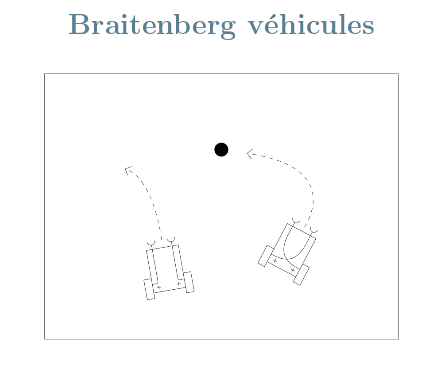
\includegraphics[width=10cm, height=10cm, keepaspectratio]{Braitenberg.png}
		\caption{Véhicule Braitenberg.}
		\label{fig:Braitenberg}
	\end{figure}
\paragraph{}	
On peut voir à travers les âges, que plusieurs civilisations (Grecques, Chine, Égypte) on modélisé leur technologies comme leurs esprits. Horloges, Systèmes hydrauliques, systèmes téléphonique, hologrammes, ordinateur analogues sont tous des métaphores de l'intelligence humaines.

\paragraph{}
Voici plusieurs événements en ordres chronologiques qui sont très important a l'IA avec une petite descriptions.
\begin{itemize}


\item \textbf{Hobbes, 1588-1679}
`Grand-Père` de l'IA. la pensée est un raisonnement symbolique. Ces idées ont été poussés par Descartes, Spinoza, Leibniz

\item \textbf{Babbage, 1792-1871}
Machine analytique, premier design d'ordinateur general-purpose

\item \textbf{Thèse Church-Turing}
Toute fonction arithmétique peut être fait sur une machine de Turing ou en calculus lambda ou formes équivalentes. n'a pas encore été prouvé mais a été testé par le temps..
\item \textbf{McCulloch et Pitts, 1943}
on prouver qu'un thresholding simple pouvait être interpréter comme une neuronne. Ce qui pourrait être une base pour une machine Turing-complete.
\item \textbf{Samuel, 1952}
Programme qui joue au checkers
\item \textbf{Minsky, 1952}
apparition du concept de réseaux de neuronnes
\item \textbf{Newell et Simon, 1956}
Programme qui trouve des preuves en logique propositionnelle.

\item \textbf{Rosenblatt, 1958}
Premier travaux significatif sur le perceptron
\item \textbf{Bobrow, 1967}
STUDENT, programme qui peut résoudre de l'algèbre de niveau secondaire en language naturel

\item \textbf{1970-1980}
Beaucoup d'effort dans les \textbf{Systèmes experts}, qui ont pour but d'avoir beaucoup de connaissances de pointes dans un domaine en particulier, pour qu'un ordinateur puisse faire des tâches de manière autonomes.
\item \textbf{Winograd, 1972}
SHRDLU, système qui peut faire une discussion et faire des actions intelligentes dans un monde simulé en utilisant que du language naturel.
\item \textbf{Warren et Pereira, 1982}
CHAT-80, peut répondre a des questions de nature géographiques en language naturel.
\item \textbf{Buchanan et Feigenbaum, 1965-1983}
DENDRAL, programme qui propose des structure atomique plausibles pour des nouveau composés organiques
\item \textbf{Buchanan et Shortliffe, 1984}
MYCIN, programme qui fait le diagnostique de maladie infectieuse du sang, prescrit le médicament requis et explique sont raisonnement
\item \textbf{1980 plus ou moins}
arrivé du prolog
\end{itemize}
\section{Agents Intelligents}
l'IA sert a utiliser un raisonnement pour faire un action. Une amalgamation d'une méthode de perception, d'un raisonnement et d'un mécanisme d'action est un \textbf{agent}. Un agent agit dans un \textbf{environnement}, les deux se trouvant dans un \textbf{monde}.
\begin{figure}[!ht]
\centering
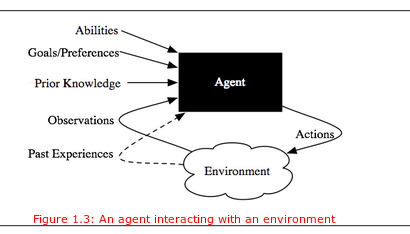
\includegraphics[width=5cm, height = 5cm, keepaspectratio]{Agent_base.png}
\caption{version generale d'un agent.}
\label{fig:Agentbase}
\end{figure}
\paragraph{}
Par exemple, un agent peut être un robot, son système de perception sont ces capteurs, sont processeur serait sa méthode de raisonnement et ses actuateurs serait sa méthode de mécanisme d'action. Son environnement serait son emplacement physique.Voici les différents types d'agents:

\begin{figure}[!ht]
\centering
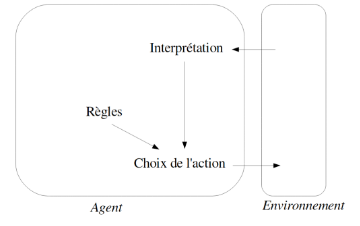
\includegraphics[width=5cm, height=5cm, keepaspectratio]{Agent_Reflexe.png}
\caption{Agent Réflexe}
\label{fig:agentreflexe}
\end{figure}
	

\begin{figure}[!ht]
\centering
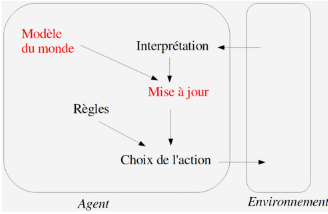
\includegraphics[width=5cm, height=5cm, keepaspectratio]{Agent_Memoire.png}
\caption{Agent Mémoire}
\label{fig:agentmem}
\end{figure}
	
\begin{figure}[!ht]
\centering
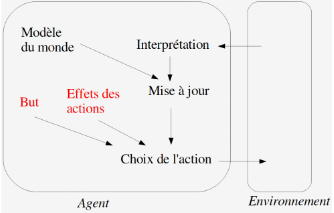
\includegraphics[width=5cm, height=5cm, keepaspectratio]{Agent_Memoire_But.png}
\caption{Agent Mémoire avec Buts}
\label{fig:agentmembut}
\end{figure}
	
\begin{figure}[!ht]
\centering
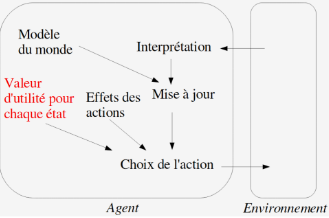
\includegraphics[width=5cm, height=5cm, keepaspectratio]{Agent_Memoire_Theorie.png}
\caption{Agent avec Théorie de la décision}
\label{fig:agenttheorie}
\end{figure}
\paragraph{}
Les agents qui peuvent apprendre sont d'une intérêt particulier. Ils peuvent eux-même changer leur comportement en fonction des échantillons d'entrainement grâces à des rétroactions positives et négatives.
\section{Méthodes de Recherche dans un Espace États}
\paragraph{État}
ou dans le monde se retrouve l'agent dans sa recherche pour la solution. C'est en fonction de chaque problême. On utilise souvent une forme arborescent pour représenter sa position.
\begin{figure}[!ht]
\centering
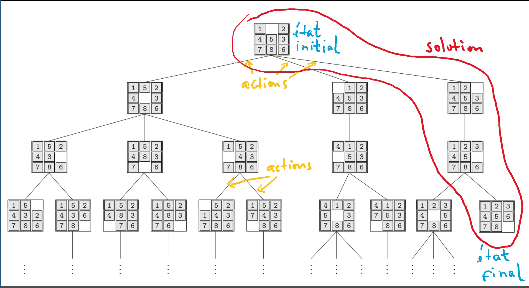
\includegraphics[width = 7cm, height = 7cm, keepaspectratio]{Etat.png}
\caption{Représentation d'un État}
\label{fig:etat}
\end{figure}

\paragraph{Fonction de Cout}
Normalement, on ne s'intéresse pas seulement a trouver une solution. On s'intéresse aussi a la qualité de la solution. On représente cela avec une fonction de cout. La convention est que le plus faible est la fonction de cout, le meilleur est la solution. Cette fonction associe une valeur a chaque action.

\paragraph{Méthode de recherche}
On définit une méthode de recherche comme étant le guideline qu'on utilise dans notre algorithme pour se déplacer dans notre espace d'états


\subsection{Méthodes de Recherche non informée}

\subsubsection{Méthode de Recherche en largeur}

\paragraph{}
La méthode de recherche en largeur cible a explorer toutes les noeuds possible de notre espace d'états sans prendre en considération la fonction de cout. Et en explorant toute les états de chaques étages de notre Arbre. Voir \ref{fig:Recherche_en_largeur} et \ref{fig:Algo_Recherche_en_largeur}

\begin{figure}[!ht]
\centering
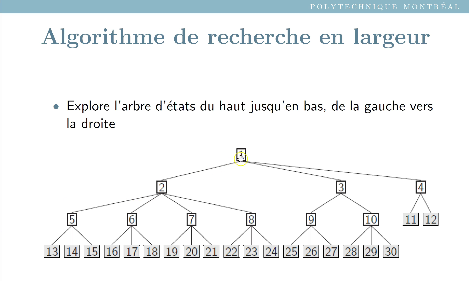
\includegraphics[width = 7cm, height = 7cm, keepaspectratio]{Recherche_Largeur.png}
\caption{Ordre d'exploration de la recherche en largeur.}
\label{fig:Recherche_en_largeur}
\end{figure}

\begin{figure}[!ht]
\centering
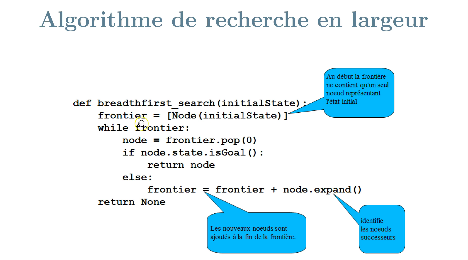
\includegraphics[width = 7cm, height = 7cm, keepaspectratio]{algo_largeur.png}
\caption{Algorithme de Recherche en Largeur.}
\label{fig:Algo_Recherche_en_largeur}
\end{figure}
\paragraph{Avantages}
on est sur d'avoir une solution. Et si tous les actions on le même cout, la solution sera optimale
\paragraph{Désavantages}
Le nombre d'état dans la frontière est très élevés.. Très grand temps de calculs et beaucoup de mémoire requis. On peut aider le problème de mémoire en prenant en considération les états déjà explorés

\subsubsection{Méthode de Recherche en profondeur}
\paragraph{}
La méthode de recherche en profondeur cible a expandre un noeud jusqu'à ce que l'état ne produit plus de nouvelle état ou qu'on trouve la solution. Si on arrive au fond. On change de branche et on commence a explorer un peu plus en largeur. Voir\ref{fig:Recherche_en_profondeur} et \ref{fig:Algo_Recherche_en_profondeur}

\begin{figure}[!ht]
\centering
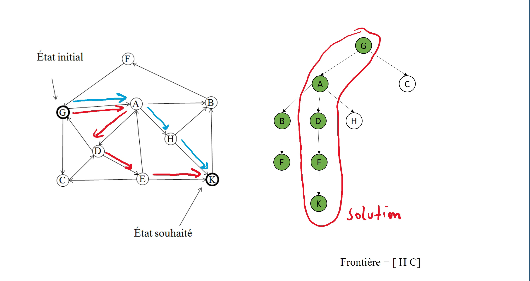
\includegraphics[width = 7cm, height = 7cm, keepaspectratio]{Recherche_Profondeur.png}
\caption{Recherche en Profondeur}
\label{fig:Recherche_en_profondeur}
\end{figure}

\begin{figure}[!ht]
\centering
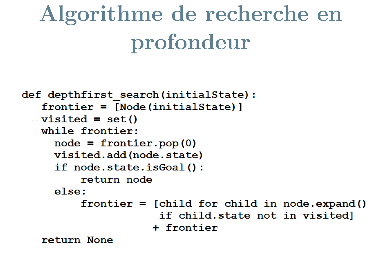
\includegraphics[width = 7cm, height = 7cm, keepaspectratio]{algo_profondeur.png}
\caption{Algorithme de Recherche en Profondeur}
\label{fig:Algo_Recherche_en_profondeur}
\end{figure}
\paragraph{Variantes Incrémentales}
On peut modifier l'algorithme de recherche en profondeur pour rectifier certains problèmes. Un des problèmes principales qu'on veut résoudre est que la recherche en profondeur peut se perdre dans une mauvaise ramification. On peut résoudre sa avec une approche incrémentale. C'est à dire, qu'on limite les solution qu'on explore en fonction de leur niveau.
\paragraph{}
Principale, on applique la recherche en profondeur avec des limites de profondeur de 1,2,3..n jusqu'à temps qu'on réussise a trouver notre solution. Sa évite que dans l'occurence qu'un problème à une très grande profondeur, qu'on se perd dans une super grande branche qui risque de ne pas donner de solution.
\paragraph{}
Cette solution n'est pas inefficace comme on l'imaginerait.. Cela est du au fait que la grande majorité du travail est fait lors du dernier niveau de l'arbre. Voir formule ci-dessous
\begin{align*}
N_{b}(D) &= \sum^D_{d=0} b^d = \frac{b^{D+1}-1}{b-1}
\end{align*}

\begin{itemize}
\centering
\item {b est le facteur de ramification}
\item {D est la profondeur de l'arbre}
\item {Nb est le nombre total de noeuds}

\end{itemize}

\subsubsection{Algorithme de Recherche a cout uniforme}

\paragraph{}
Les méthode de recherches en profondeur et en largeur ont tous les deux de grands désavantages qui rendent ces méthodes inutiles pour certains problèmes spécifiques. De plus, les deux algorithmes ne trouvent pas nécessairement la solution optimale.

\paragraph{}
L'algorithme de recherche à cout uniforme, malgré son nom un peu confusing, prend en compte de la fonction de cout. Fonction qui n'a pas nécessairement un cout uniforme.. \\

l'algorithme va toujours vouloir chercher les noeuds ayant une somme de couts minimales. Cette méthode va toujours donner une solution optimale. Par contre, elle risque d'explorer autant de noeuds que les méthodes de recherche en profondeur et en largeur. On peut considérer la recherche en largeur comme étant un cas particulier de la recherche a cout uniforme, si et seulement si la fonction de cout est égale pour chaque actions. Voir \ref{fig:Algo_Recherche_Uniforme} et \ref{fig:Recherche_Uniforme}

\begin{figure}[!ht]
\centering
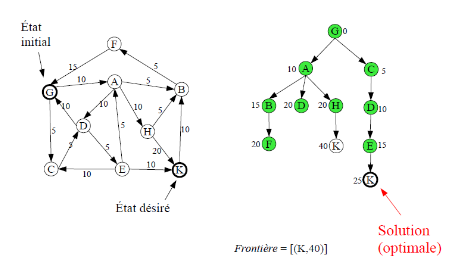
\includegraphics[width = 7cm, height = 7cm, keepaspectratio]{Recherche_Uniforme.png}
\caption{Recherche à cout Uniforme}
\label{fig:Recherche_Uniforme}
\end{figure}

\begin{figure}[!ht]
\centering
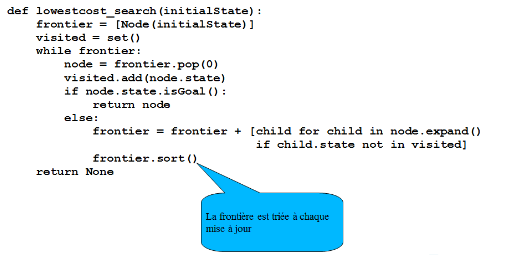
\includegraphics[width = 7cm, height = 7cm, keepaspectratio]{algo_uniforme.png}
\caption{Algorithme de Recherche a cout Uniforme}
\label{fig:Algo_Recherche_Uniforme}
\end{figure}

\subsubsection{Recherche Bidirectionel}
\paragraph{}
N'étant pas nécessairement un algorithme de recherche, la recherche bidirectionel est une facon de réduire le temps de recherche si on respect certain critères.
\begin{itemize}
\item Si on a une solution possible.
\item Si c'est possible de se rendre a la solution à partir de notre état d'origine, sinon notre solution et nos état initiale ne vont jamais converger.
\end{itemize}
 L'idée derrière la recherche bidirectionel est qu'on utilise notre algorithme de recherche dans les deux sens. Une fois en partant de l'origine pour se rendre jusqu'à la solution connus. La deuxième en partant de la solution pour essayer de se rendre jusqu'à l'état d'origine. \\
 
Normalement, on utilise une combinaison d'algorithme de recherche en profondeur partant de la solution et d'algorithme de recherche en largeur qui part de l'origine. Notre algorithme d'origine cherche a approfondire la frontière de noeud le plus largemene possible tandis que l'algorithme de notre solution cherche a la traversé. \\

Dans certains cas, nous allons avoir une amélioration. On peut la modélisé comme étant:
\begin{align*}
O_{initiale} &= b^{k} \\
O_{bidirectionel} &= 2b^{\frac{k}{2}}
\end{align*}
\begin{center}
ou b est le facteur de branchement et k la profondeur
\end{center}

\paragraph{}
Cependant, on assume toujours que nous sommes capables de rejoindre les frontières, ce qui n'est pas toujours le cas....

\subsection{Méthode de Recherche Informée}
\paragraph{Heuristique}
Une heuristique est une fonction qui essaie d'évaluer le potentiel d'un état donné en fonction de charactéristique distinctes à cet état. Ne pas confondre avec la fonction de cout, Celle-ci calcule le cout de l'état d'origine jusqu'à l'état actuel tandis que l'heuristique essaie d'estimer le cout de l'état actuel jusqu'à la solution.
\paragraph{}

par contre..
\begin{itemize}
\item Ce n'est pas garantie
\item Il faut que l'heuristique soit valide
\end{itemize}

On va s'en servir en l'incorporant dans notre algorithme de recherche, on va utiliser la fonction d'évaluation heuristique avec notre fonction de cout.\\

Pour trouver une bonne fonctions heuristiques, on peut soit parler avec un experts pour savoir quel sont les paramêtres les plus importants/qui peuvent être exploiter. \\

encore mieux, on peut aussi se servir de \textbf{l'apprentissage machine} pour pouvoir trouver nos paramêtre les plus statistiquement significatifs. Notre algorithme pourrait même ajuster son heuristique en fonction de sa.

\subsubsection{Heuristique Glutone}
\paragraph{}
Cet algorithme ne prend que l'heuristique en considération. On va s'en servir comme l'algorithme de recherche a cout uniforme sauf qu'au lieu de minimiser la fonction de cout, on va changer de voisins en prenant le voisins ayant l'heuristique la plus faible. Voir \ref{fig:Heuristique_Glutone} et \ref{fig:Prob_Heuristique_Glutone}

\begin{figure}[!ht]
\centering
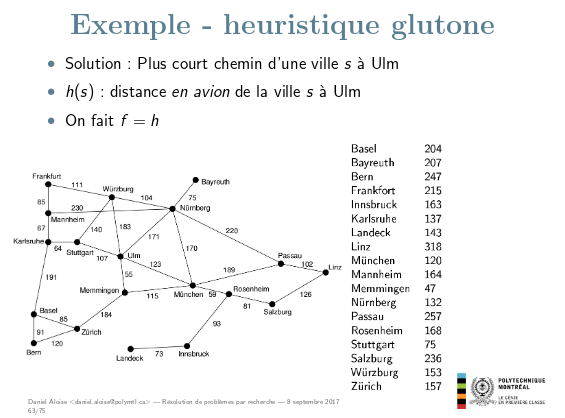
\includegraphics[width = 7cm, height = 7cm, keepaspectratio]{Heuristique_Glutone_Prob.png}
\caption{Problème d'heuristique glutone}
\label{fig:Prob_Heuristique_Glutone}
\end{figure}

\begin{figure}[!ht]
\centering
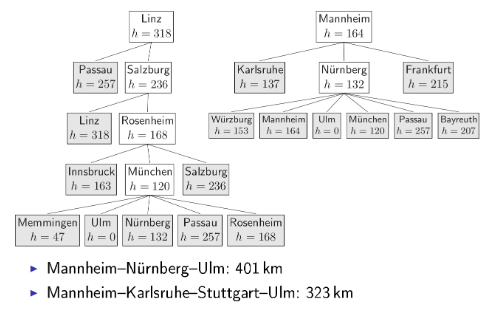
\includegraphics[width = 7cm, height = 7cm, keepaspectratio]{Heuristique_Glutone.png}
\caption{Prise de Décision de notre Heuristique Glutone}
\label{fig:Heuristique_Glutone}
\end{figure}

\subsubsection{Algorithme A*}
\paragraph{}
C'est algorithme ressemble grandement à l'algorithme de Recherche à cout uniforme. Cependant. Nous n'allons pas optimiser la fonction de cout, mais une fonction $f$ que nous allons définir comme étant
\begin{align*}
f(n) &= g(n) + h(n)
\end{align*}
\begin{center}
ou $g$ est notre fonction de cout défini dans la méthode de recherche a cout uniforme et $h$ comme étant notre heuristique. 
\end{center}


\paragraph{}
On peut alors déduire, qu'avec $h(n) = 0$ nous avons une recherche a cout uniforme et qu'avec $g(n) = 0$ nous avons une heuristique glutone. Voir fig.

\begin{figure}[!ht]
	\centering
	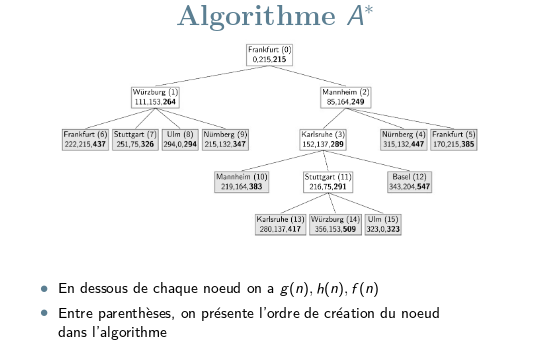
\includegraphics[width = 7cm, height = 7cm, keepaspectratio]{A*.png}
	\caption{Algorithme A*}
	\label{fig:A*}
\end{figure}
\paragraph{}
Par contre, pour que notre algorithme trouve une solution optimale, il faut que notre heuristique soit admissible. Soit:
\begin{align*}
g(x) = g(x) + h(x) \\
f(x) \leq f(z) \\
= f(x)\\
\leq f(z) \\
\leq g(z) + h(z) \leq g(y)
\end{align*}
pour fig\ref{fig:Preuve_A*}
\begin{figure}[!ht]
\centering
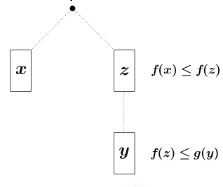
\includegraphics[width = 7cm, height = 7cm, keepaspectratio]{Preuve_A*.png}
\caption{Notre preuve pour A*}
\label{fig:Preuve_A*}
\end{figure}
\paragraph{}
Les faiblesse de l'algorithme A* sont 
\begin{itemize}
\item On peut avoir un grand nombre de noeuds à stocker
\item On doit les trier en plus à chaque itération (beaucoup de temps de calculs)
\end{itemize}
Pour régler ce problème, nous allons utiliser une recherche incrémentales.
\subsubsection{Variante A* incrémentale}
\paragraph{}
Cette variante est comme la recherche en profondeur incrémentale sauf qu'au lieu de limiter la profondeur, nous allons limiter la valeur de la fonction $f(n)$. Voir les figures 

\begin{figure}[!ht]
\centering
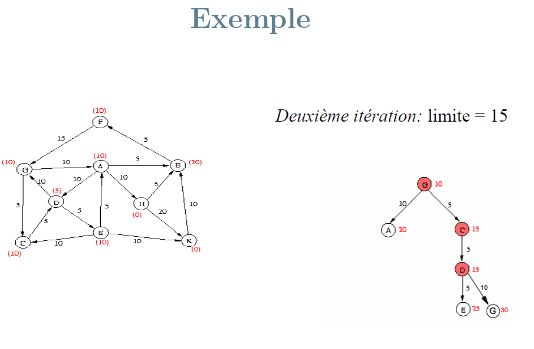
\includegraphics[width = 7cm, height = 7cm, keepaspectratio]{incrementale_15.png}
\caption{Limite de 15 dans l'approche incrémentale}
\label{fig:incrementale15}
\end{figure}

\begin{figure}[!ht]
\centering
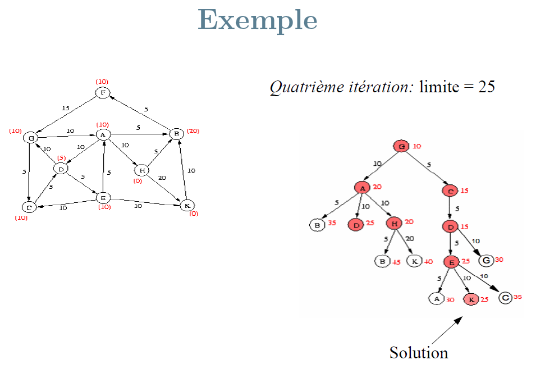
\includegraphics[width = 7cm, height = 7cm, keepaspectratio]{incrementale_25.png}
\caption{Limite de 25 dans l'approche incrémentale}
\label{fig:incrementale25}
\end{figure}
\subsection{Méthode de Recherche Locale}
\paragraph{Voisinage}
On appel un voisinage tous les noeuds qui peuvent être un successeur de l'état en question. pour revenir à notre analogie arborescente, le voisinage de l'état initiale serait l'étage en dessous. Le voisinage de tous les états du première étage serait les états du deuxième étage.. ainsi de suite.\\

Les méthodes de recherche locales ne conservent qu'un seul noeud en mémoire, celui ou nous sommes. En générale, avec une méthode de recherche locale on cherche seulement à trouver une solution, et non pas comment se rendre à la solution selon notre origine.\\

À chaque itération de notre algorithme, on remplace par notre meilleur noeuds jusqu'à temps qu'on a une solution.

\end{document}
